% arara: pdflatex: { shell: yes }

\documentclass[border=3pt]{standalone}  % see standalone package doc
\usepackage[utf8]{inputenc}
\usepackage{tikz}
\usetikzlibrary{mindmap,shadows}


%\definecolor{mygold}{HTML}{ffc61e}
%\definecolor{mypurple}{HTML}{af58ba}
%\definecolor{myblue}{HTML}{009ade}
%\definecolor{mygreen}{HTML}{00cd6c}


\definecolor{myblue1}{HTML}{0000FF}
\definecolor{myblue2}{HTML}{0066FF}
\definecolor{myblue3}{HTML}{3388FF}
\definecolor{myblue4}{HTML}{77ccff}


\begin{document}
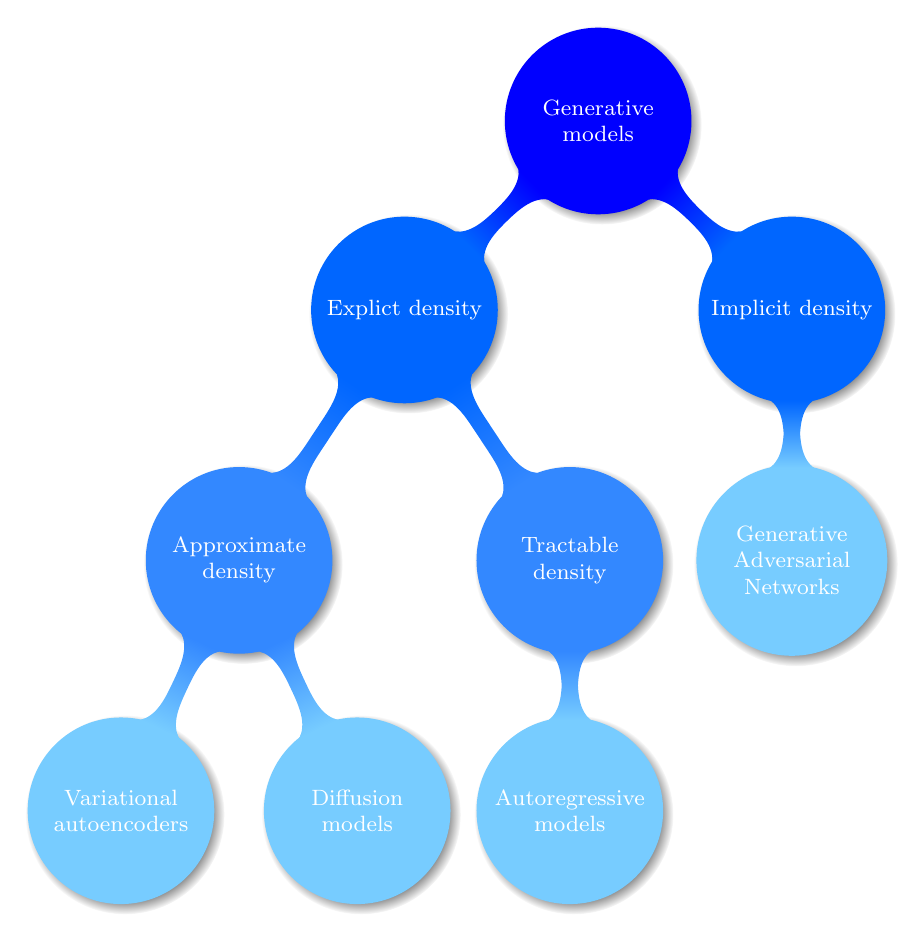
\begin{tikzpicture}[small mindmap,every node/.style={concept,circular drop shadow}, 
                    concept color=myblue1,text=white,
                    level 1/.style={level distance=4cm, sibling distance=8.2cm},
                    level 2/.style={level distance=5.3cm, sibling distance=7cm},
                    level 3/.style={level distance=5.3cm, sibling distance=5cm}]                    
\node{Generative models}
    child [concept color=myblue2, scale = 0.6]  { node {Explict density}
        child [concept color=myblue3] { node {Approximate density}
            child[concept color=myblue4] { node {Variational autoencoders}}
            child[concept color=myblue4] { node {Diffusion models}} 
        }
        child [concept color=myblue3] { node {Tractable density}
            child[concept color=myblue4] { node {Autoregressive models}} 
        }
    }
    child [concept color=myblue2,  scale = 0.6]{ node {Implicit density}
	    child [concept color=myblue4] { node {Generative Adversarial Networks}}
    };
\end{tikzpicture}
\end{document}